\documentclass{beamer}
\usepackage{ctex}
\usepackage{hyperref}
\usepackage{calligra}
\usepackage[T1]{fontenc}
\usepackage{ncepu}
\usepackage{graphicx}
% \usepackage[utf8]{inputenc} 
% \usepackage{fontspec}
% \setmainfont{Times New Roman}

\definecolor{ncepu_blue}{RGB}{0,90,160}

\author{林新辉}
\title{基于数据驱动方法的动力电池健康状态估计和剩余寿命预测方法研究}
\subtitle{Research on Data-Driven Approaches for Estimating Health Status and Predicting Remaining Useful Life of Lithium-Ion Batteries in Electric Vehicles}
\institute{控制与计算机工程学院,华北电力大学}
\date{2023年6月13日}


\begin{document}

% 封面页
\kaishu
\begin{frame}
\titlepage
\end{frame}

% 目录页
\begin{frame}
\tableofcontents[sectionstyle=show,subsectionstyle=show/shaded/hide,subsubsectionstyle=show/shaded/hide]
\end{frame}

\section{研究背景和研究对象}

\begin{frame}
	\begin{figure}[htbp]
		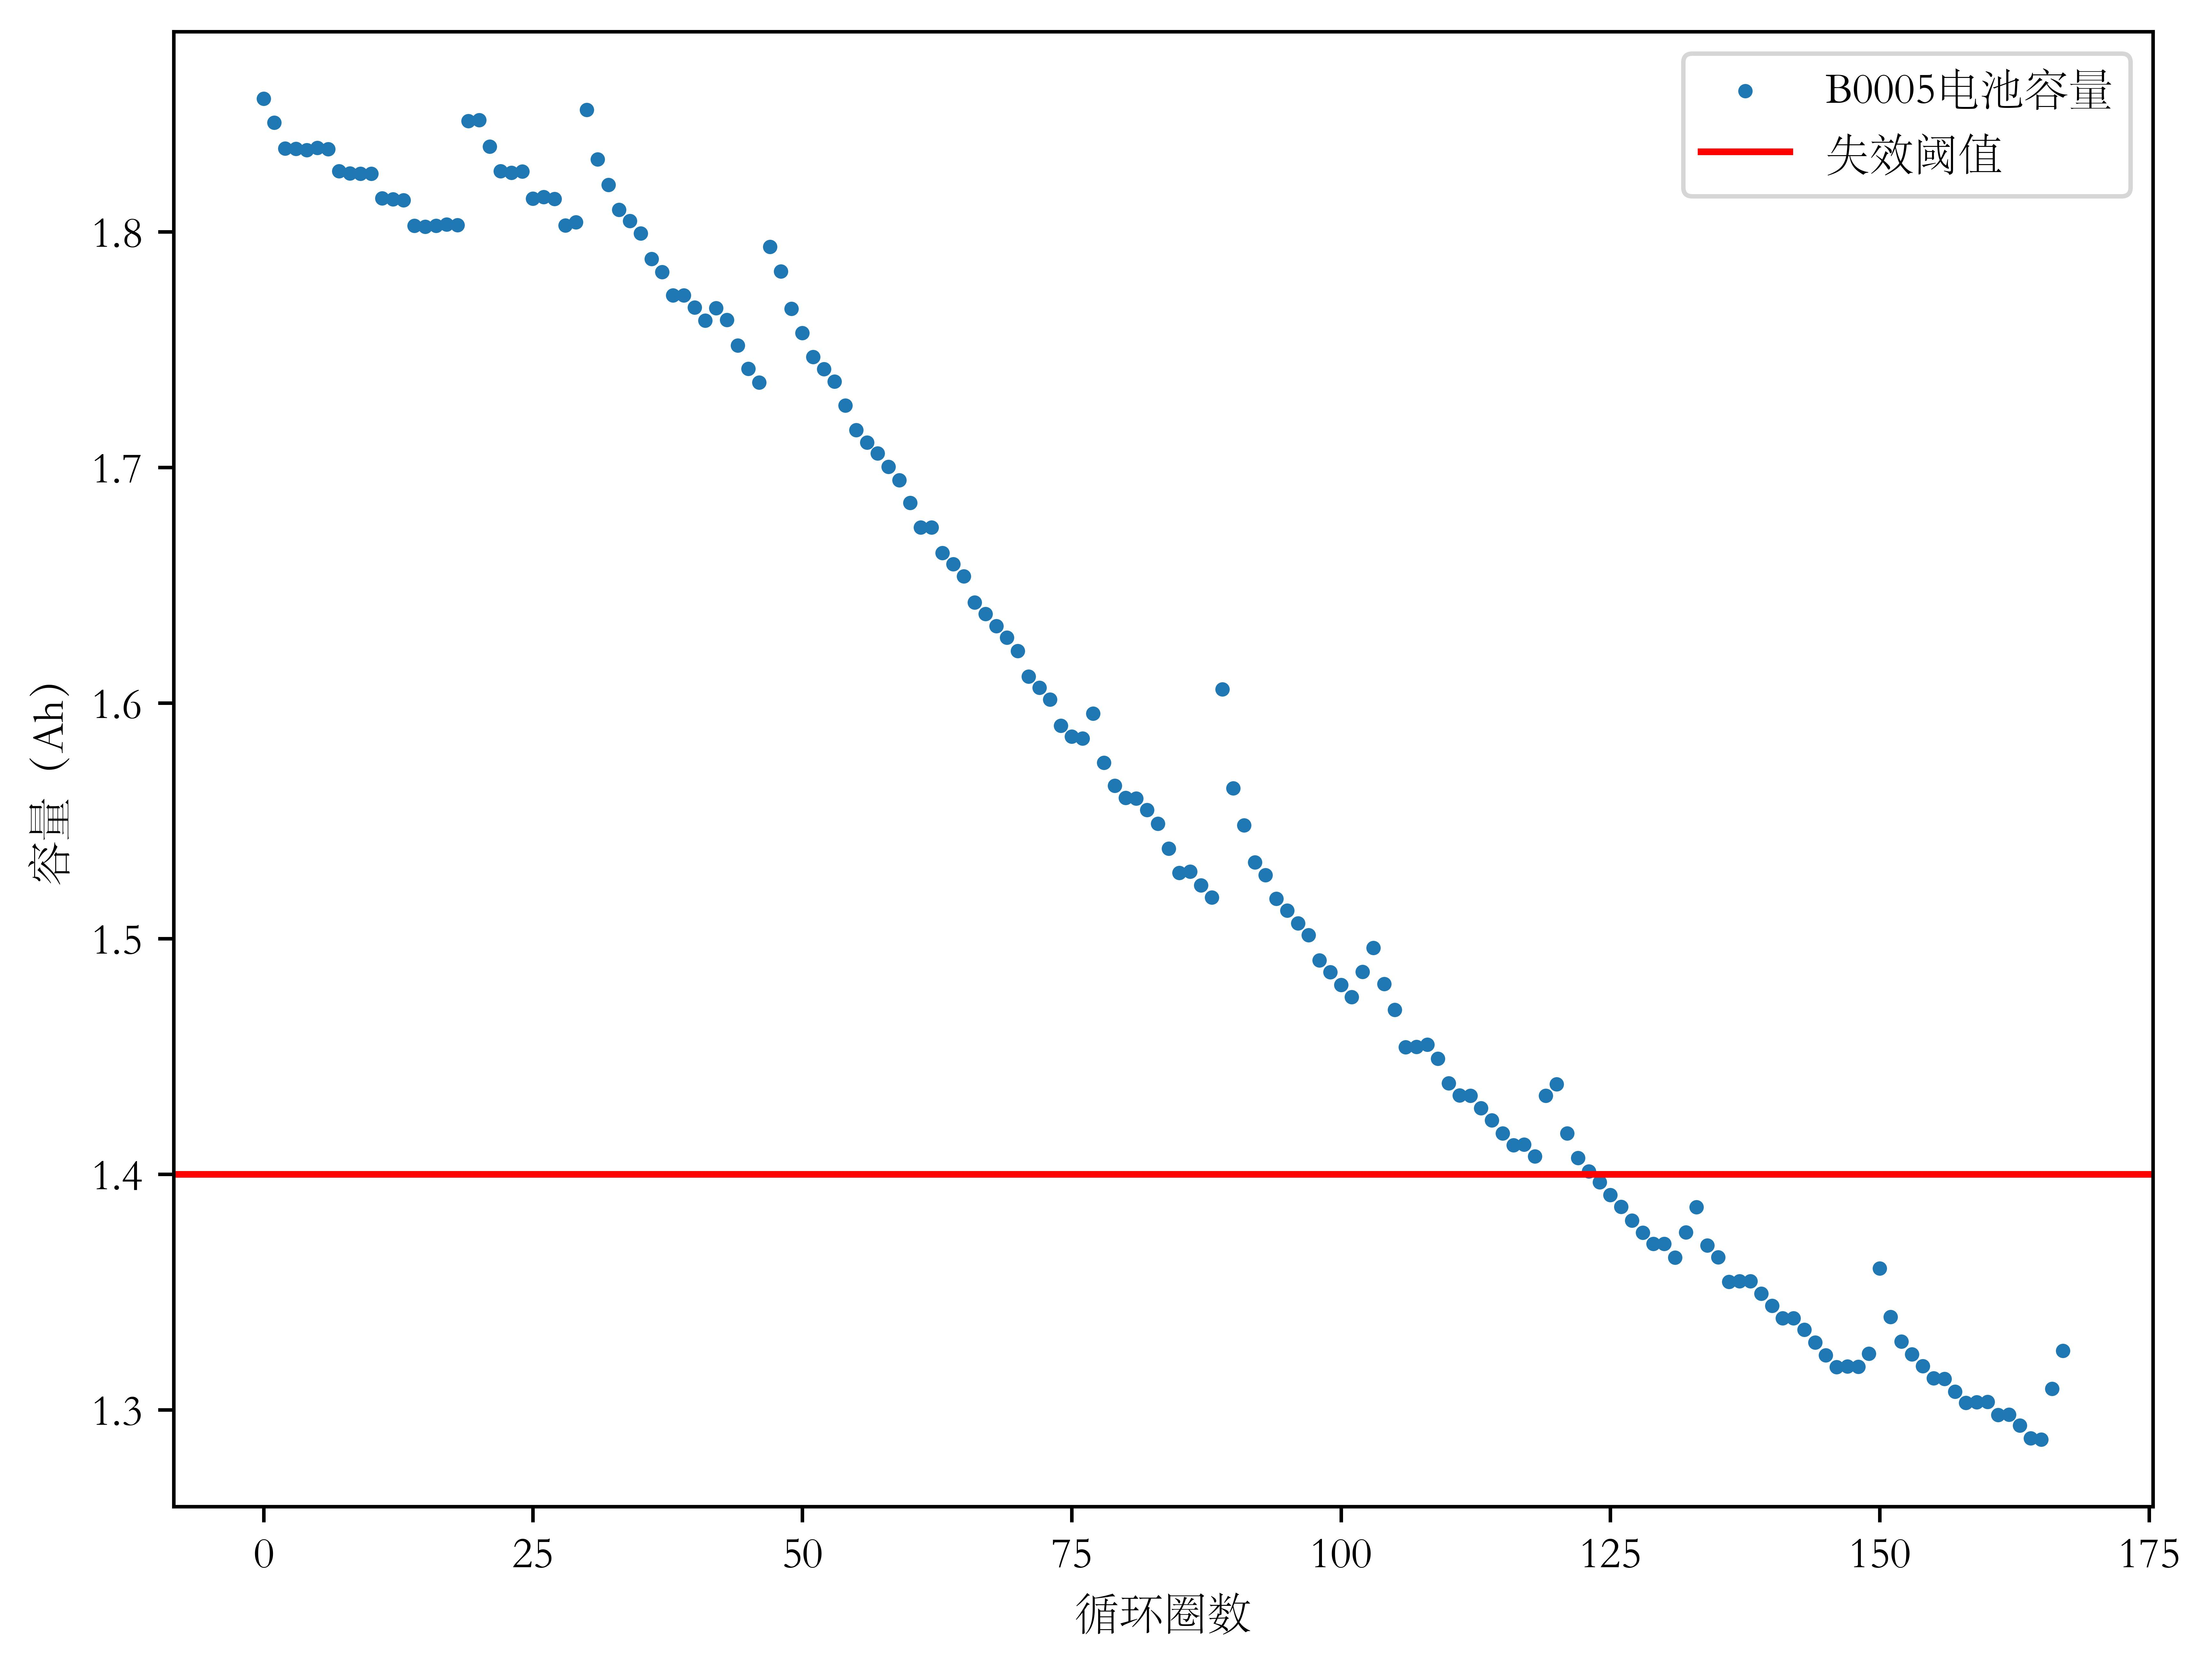
\includegraphics[scale=0.5]{figures/nasa_B0005_failure_threshold.jpg}
	\end{figure}
\end{frame}

\section{建模和实验}

\subsection{基于电池容量历史退化数据的SOH估计}

\begin{frame}
	\begin{itemize}
		\item 五个模型均取得较高预测精度,使用数据驱动方法实现锂离子电池SOH估计具有可行性
		\item 对于短时预测问题,非隐状态模型的预测精度高于隐状态模型
	\end{itemize}
\end{frame}

\subsection{基于电池充放电直接测量量的SOH估计}

\begin{frame}
	\begin{itemize}
		\item 对比使用V、I、T为输入的情形,使用V、I、SOC为输入时模型预测结果有很大提升
		\item 使用时间序列-图像变换能在保持预测精度的前提下显著降低模型参数量
	\end{itemize}
\end{frame}

\subsection{电池RUL预测}

\begin{frame}
	% \begin{itemize}
	% \end{itemize}
	实验结果表明使用数据驱动方法实现锂离子电池RUL预测具有可行性
\end{frame}

\section{展望}

\begin{frame}
	\begin{itemize}
		\item 估计/预测模型改进
			\begin{itemize}
				\item 融合机理模型和数据驱动模型,提高模型性能
				\item 引入贝叶斯模型,实现对预测结果的不确定性度量以更好支持工业决策
				\item 引入迁移学习,提高模型泛化能力
			\end{itemize}
		\item 模型在嵌入式平台的部署:模型量化和模型转换
	\end{itemize}
\end{frame}

\section{写在最后}

\begin{frame}
	\centering
	本课题相关代码已在github上开源

	\centering
	\url {https://github.com/hilinxinhui/battery_phm.git}

	\begin{figure}[htbp]
		\centering
		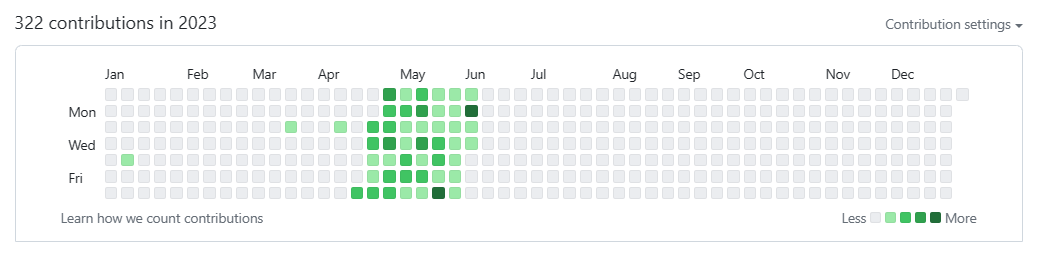
\includegraphics[scale=0.3]{figures/github_contribution_log.png}
	\end{figure}

	\begin{figure}[htbp]
		\centering
		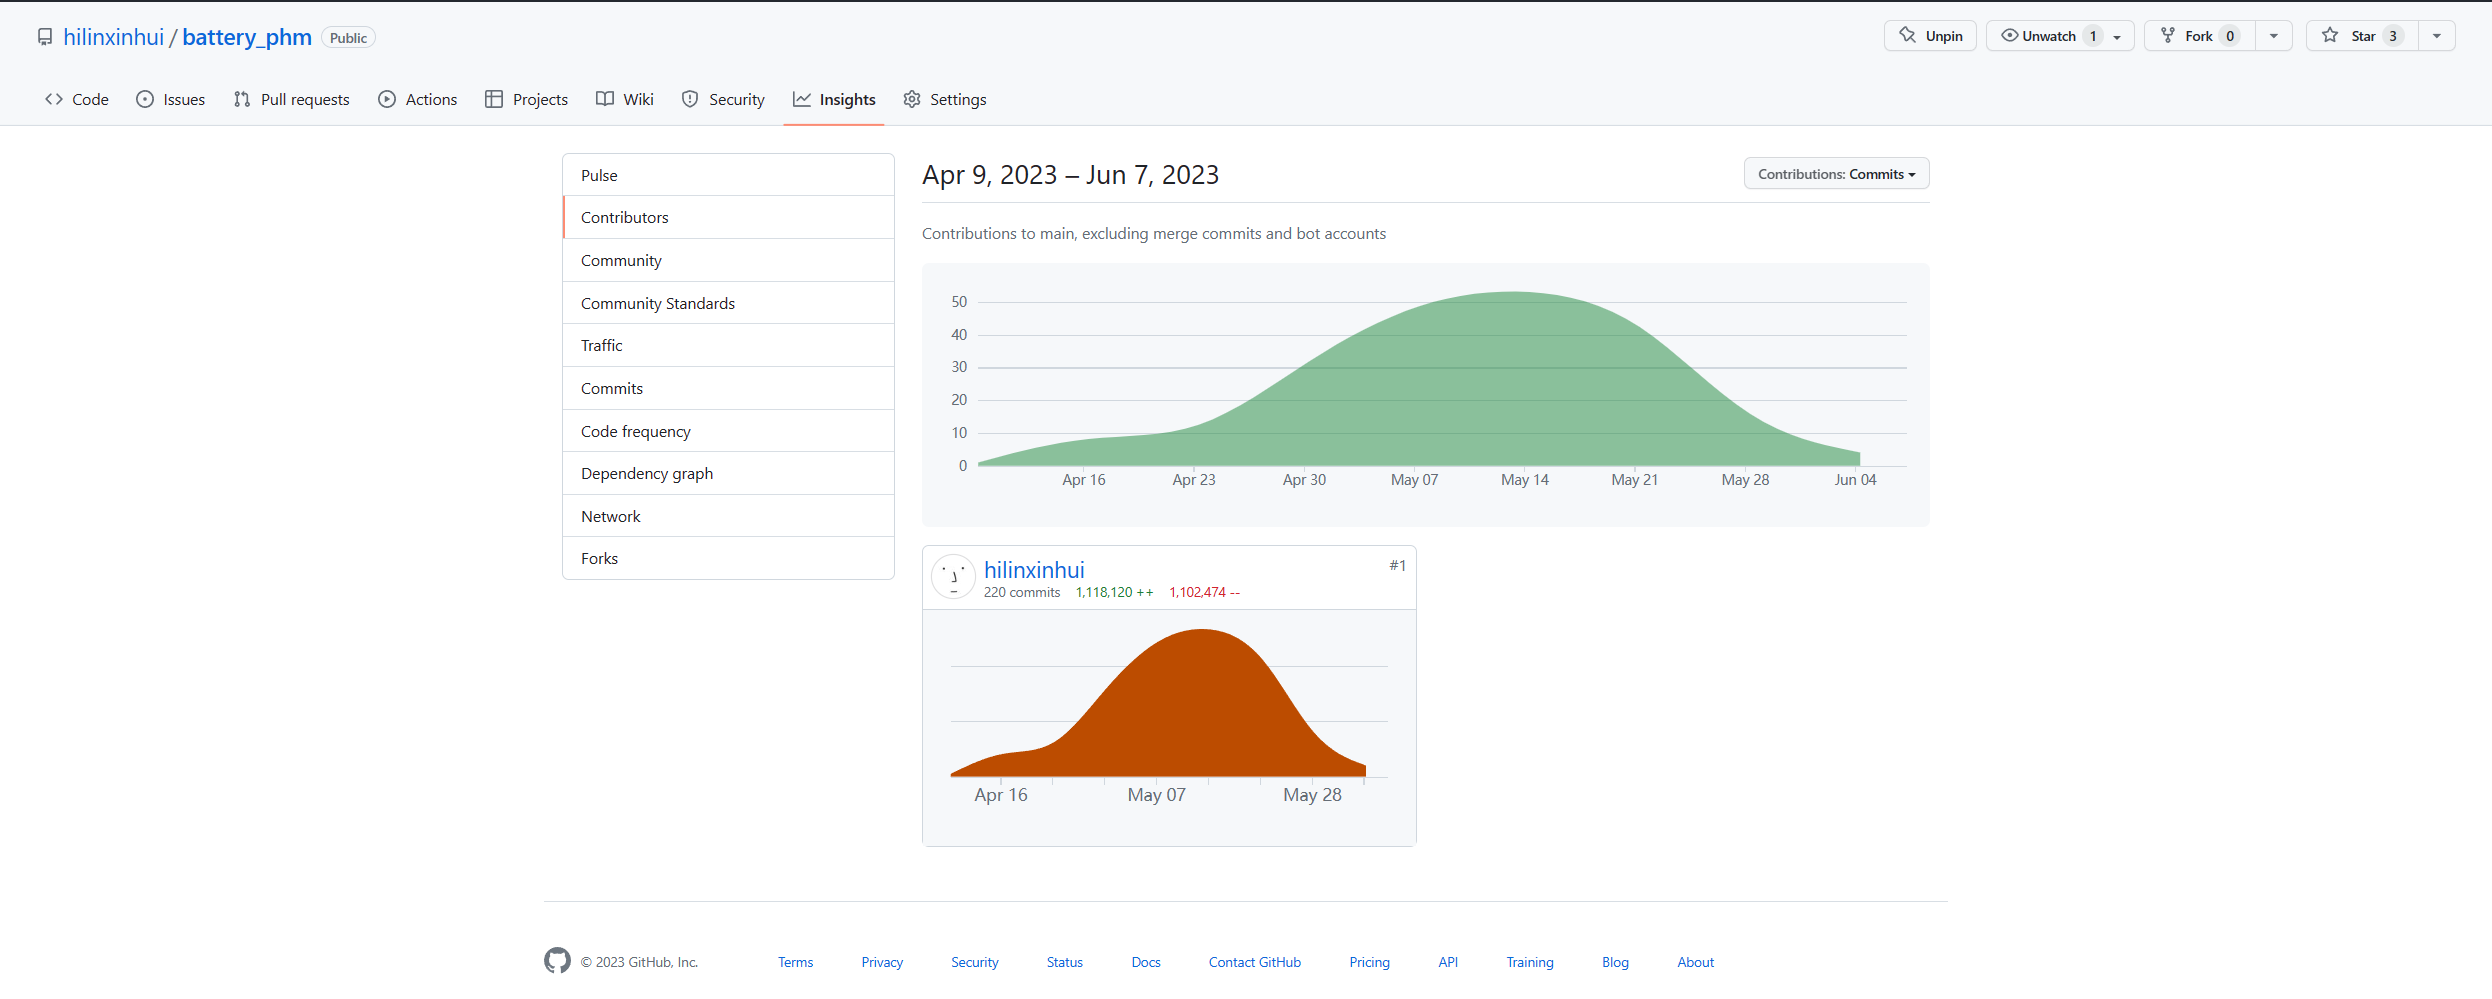
\includegraphics[scale=0.15]{figures/github_contribution_log_2.png}
	\end{figure}

\end{frame}

\begin{frame}
	\LARGE \centering 汇报完毕,请各位老师批评指正!
\end{frame}

\end{document}
